\documentclass{article}
\usepackage{hyperref}
\usepackage{pdfpages}
\title{EMISY Project 21 Portable Compass}
\author{Krzysztof Rudnicki, 307585}
\date{\today}
\begin{document}
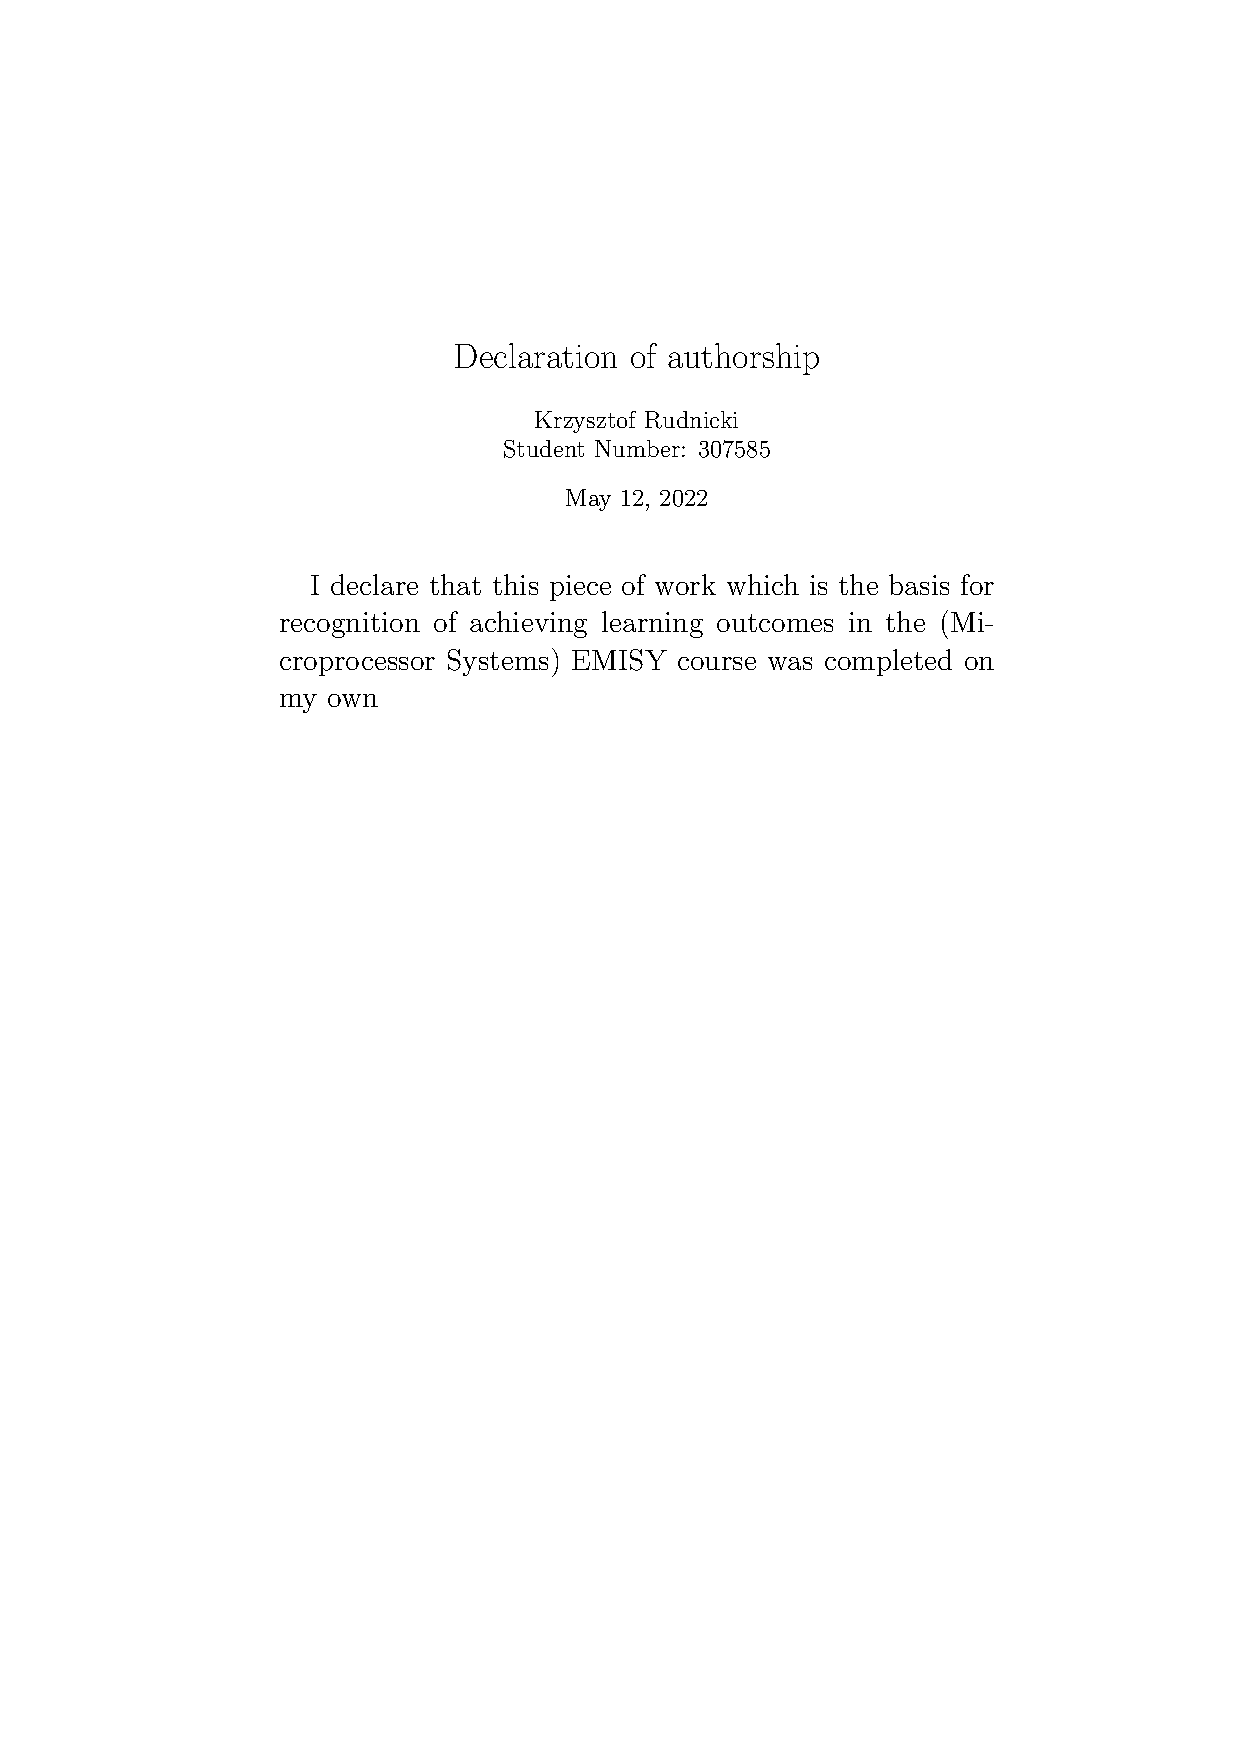
\includepdf[pages={1}]{declaration.pdf}
\maketitle
\section{Analysis of the project}
\subsection{Discussion of project requirements}
We need to create a simple portable compass circuit \\
It should:
\begin{itemize}
	\item Use energy-saving power modes of microcontroller
	\item Be battery powered
	\item Be portable (cellphone/wrist watch)
	\item Communicate using graphical OLED display and two buttons keyboard
\end{itemize}
\subsection{Discussion of solution}
\section{Detailed circuit diagram}
\section{Diagram}
\subsection{Diagram itself}
\subsection{Diagram description}
\subsubsection{How to make the project}
\newpage
\subsubsection{Microcontroller}
I decided to use STM32L082CZ from STM32L0 line
\paragraph{Relatively small} Up to 10 mm $\times$ 10 mm dimensions, 
compared to apple watch display of 34 mm by 40 mm for smaller version. 
\cite{datasheet}
111th page
\paragraph{Square} It is shaped in a square which also simplifies portability
\cite{datasheet} 111th page
\paragraph{Power saving} STM32L0 line was designed specifically for low power
consumption with power consumption as low as 0.29 $\mi$ A in Standby mode
\cite{datasheet} 1st page
\paragraph{Consumer devices} This microcontroller comes from STM32LOx2 line
prepared to be used in consumer devices \cite{consumerDevice}
\paragraph{Ease of use} USB compatible microcontroller and dedicaded debug port
allows for swift code creation.
\cite{datasheet} 1st page 
\subsubsection{All other components}
\section{Draft of the microcontroller firmware}
\subsection{Block diagram}
\subsection{Description of the algorithm}
\begin{thebibliography}{9}
	\bibitem{datasheet} 
	\href{https://www.st.com/resource/en/datasheet/stm32l082cz.pdf}{STM32LO82CZ
	datasheet}
	\bibitem{consumerDevice}
	\href{https://www.st.com/en/microcontrollers-microprocessors/stm32l0-series.html}{Consumer
	Device STM32LOx2 Line}
\end{thebibliography}
\end{document}

